\chapter{Data Collection}\label{ch:data-collection}

The ArduPilot software has an active community consisting of users and developers.
They have three different sources to exchange their knowledge, ask for help or get information about the system.
Unfortunately, the channels differ significantly in the availability of their content.
Therefore, we decided to provide a tailored web scraping solution for each channel.


\section{Discussion Forum}\label{sec:discussion-forum}
The discussion forum is the mainly used community channel of ArduPilot.
Users and developers can inform, discuss and ask questions about topics in the domain of \ac{UAV} systems.
This section aims to provide a methodology to build a tailored web scraper for the discussion forum.

\subsection{Structure Of The Forum}\label{subsec:structure-of-the-forum}
\begin{figure}
    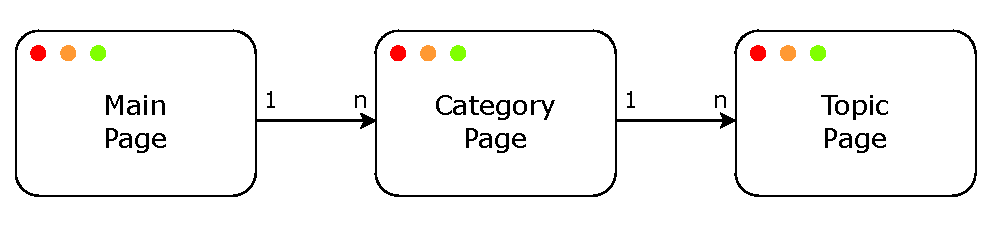
\includegraphics[width=\textwidth]{figures/data_collection/forum_structure}
    \caption{Page Structure of the Discussion Forum}\label{fig:forum-structure}
\end{figure}
First, we analyze the page structure of the forum.
In \autoref{fig:forum-structure} we can see the structure of the forum, which consists of three layers and builds a hierarchical tree.

\subsubsection{Main Page}
\begin{figure}
    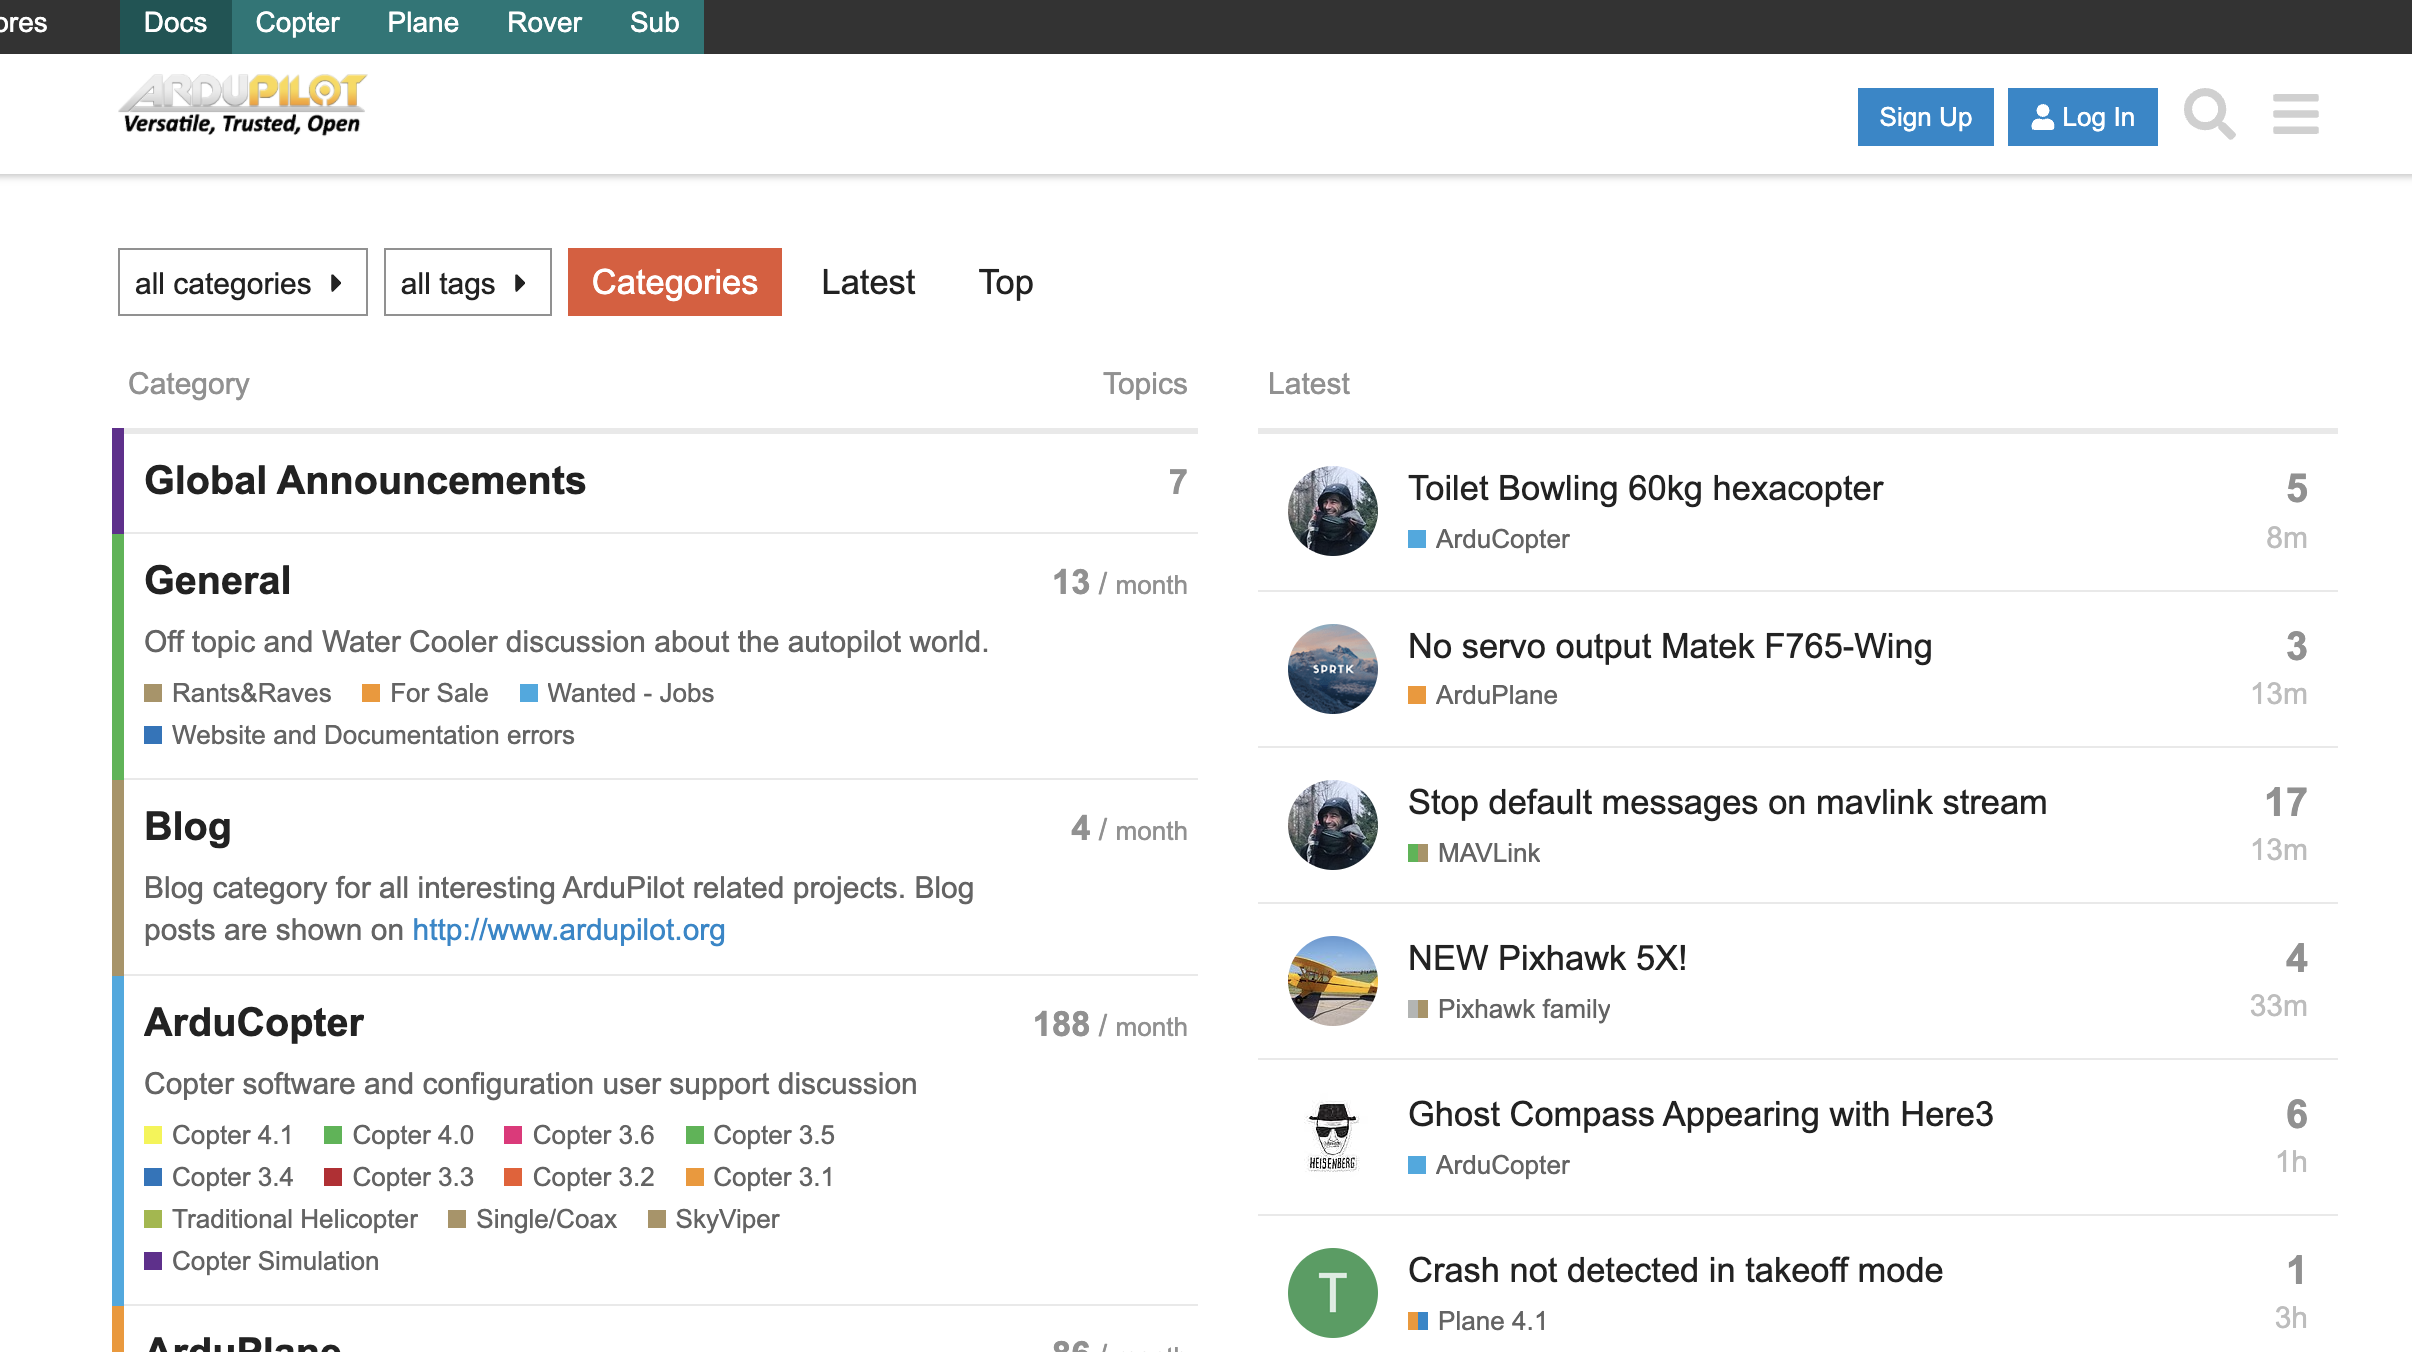
\includegraphics[width=\textwidth]{figures/data_collection/forum_main_page}
    \caption{Main Page}\label{fig:forum-main-page}
\end{figure}
The main page is the root of the structure and the starting point when joining the discussion forum.
In \autoref{fig:forum-main-page} we can see the page from the perspective of a user.
This page gives an overview of all available categories in the forum and links to the corresponding category pages.

\subsubsection{Category Page}
\begin{figure}
    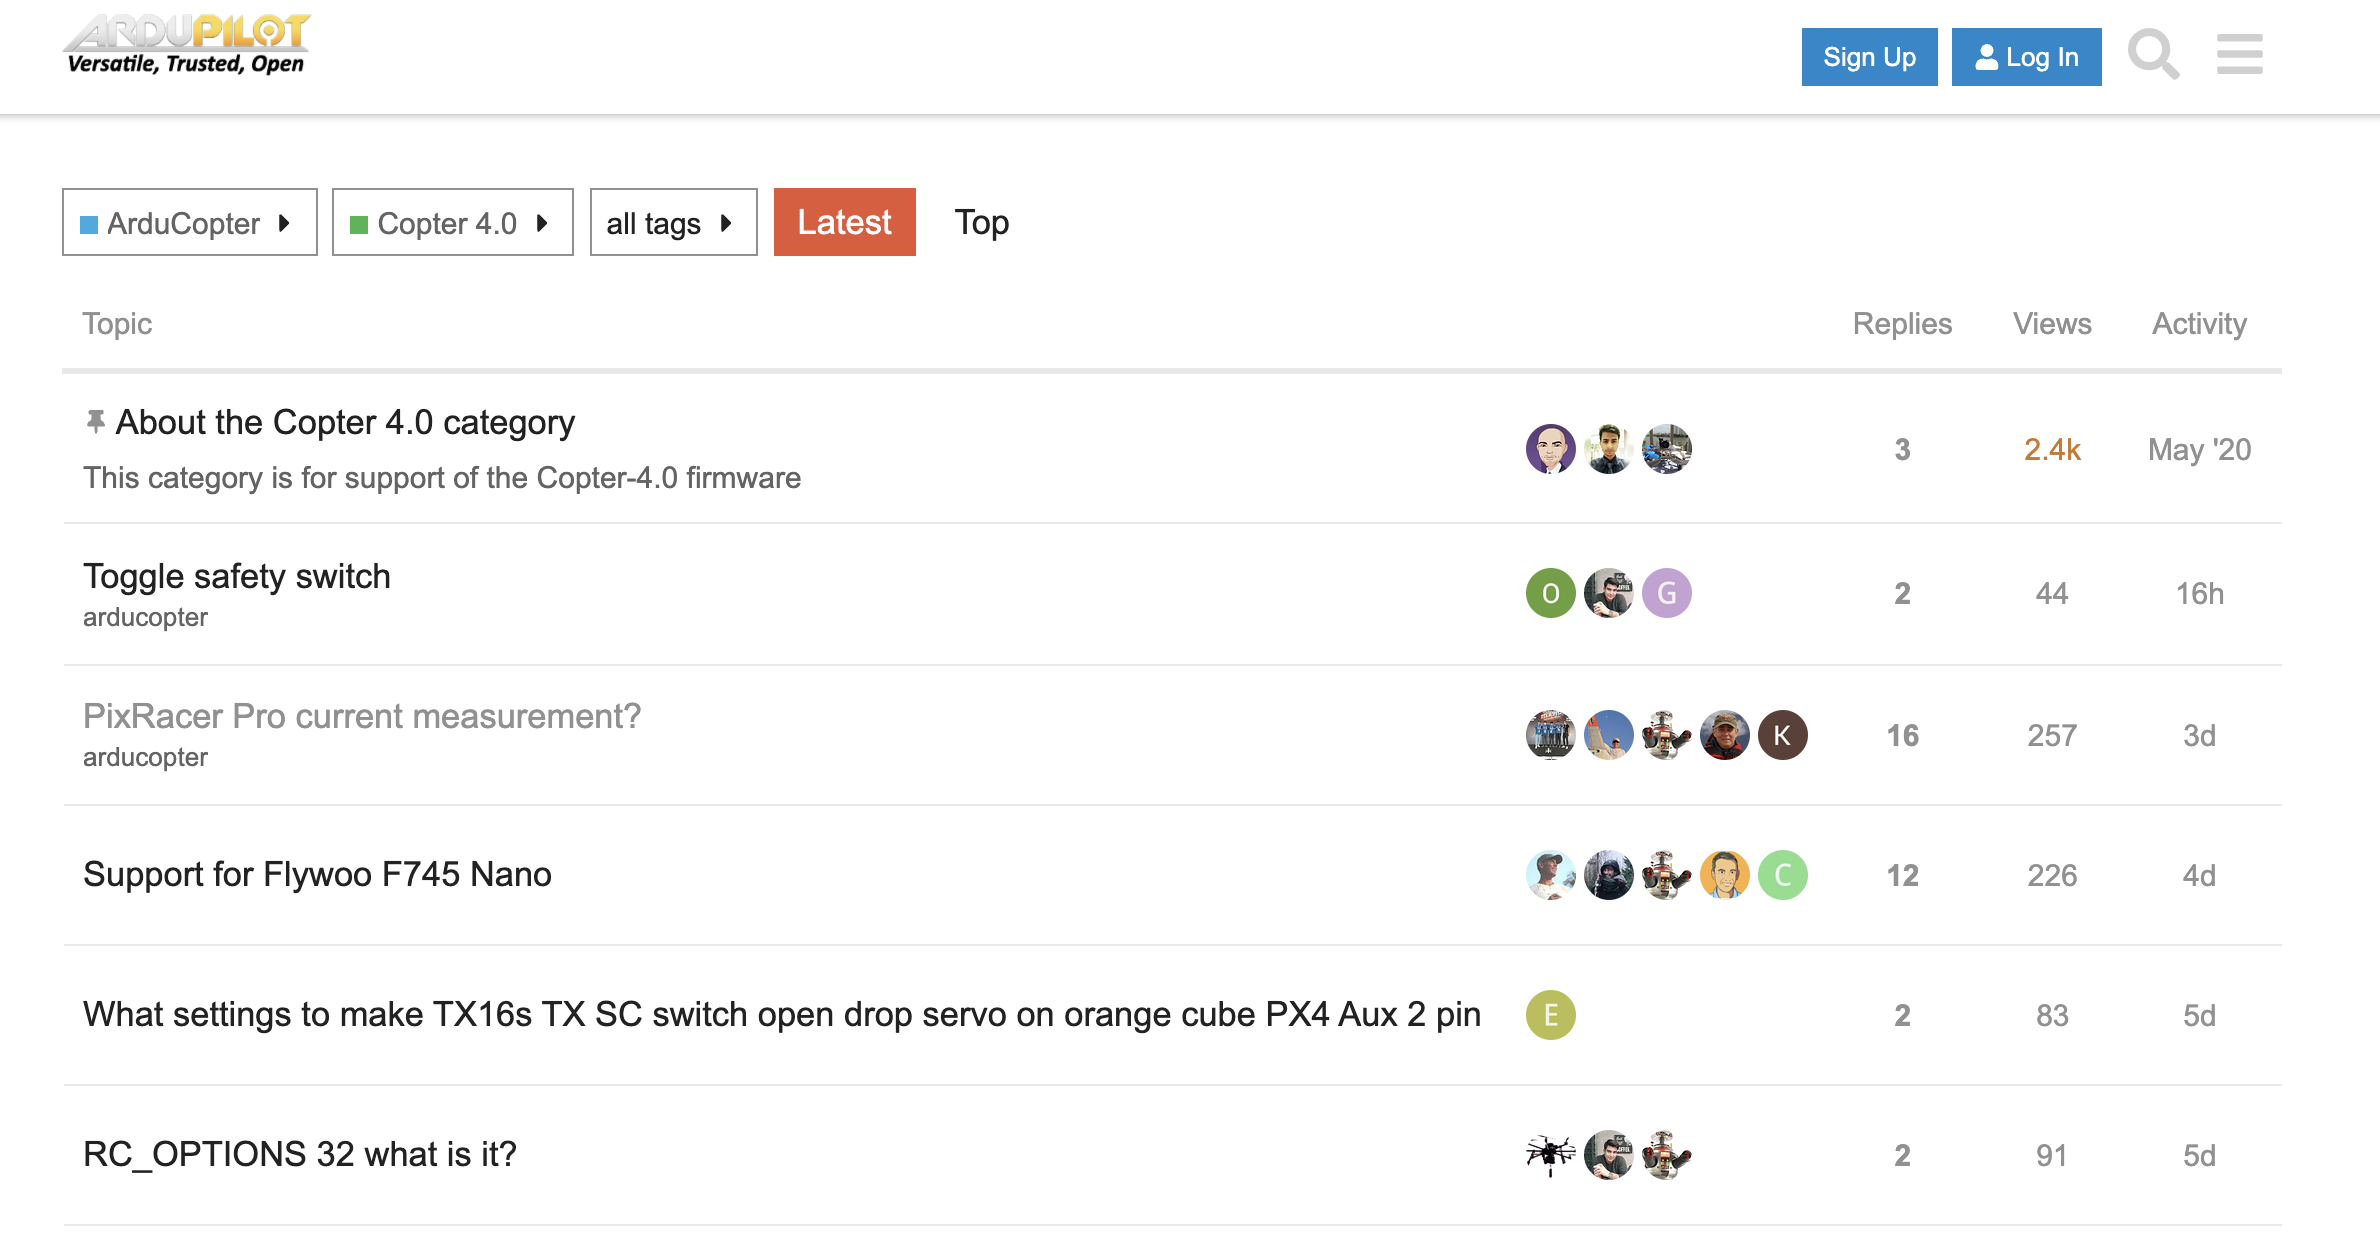
\includegraphics[width=\textwidth]{figures/data_collection/forum_category_page}
    \caption{Category Page}\label{fig:forum-category-page}
\end{figure}
The second layer is the category page, which gives an overview of all topics discussed in that category.
In \autoref{fig:forum-category-page}, we can see the category page for the root category \qq{ArduCopter} with the subcategory \qq{Copter 4.0}.
This page lists all topics linked to that category.
Additionally, different information is accessible for each topic, such as the number of users' replies, the count of the views for a topic, or the last activity.
Since such a page can have thousands of topics, the page loads new topics dynamically when a user scrolls at the bottom of the page.

\subsubsection{Topic Page}
\begin{figure}
    \begin{center}
        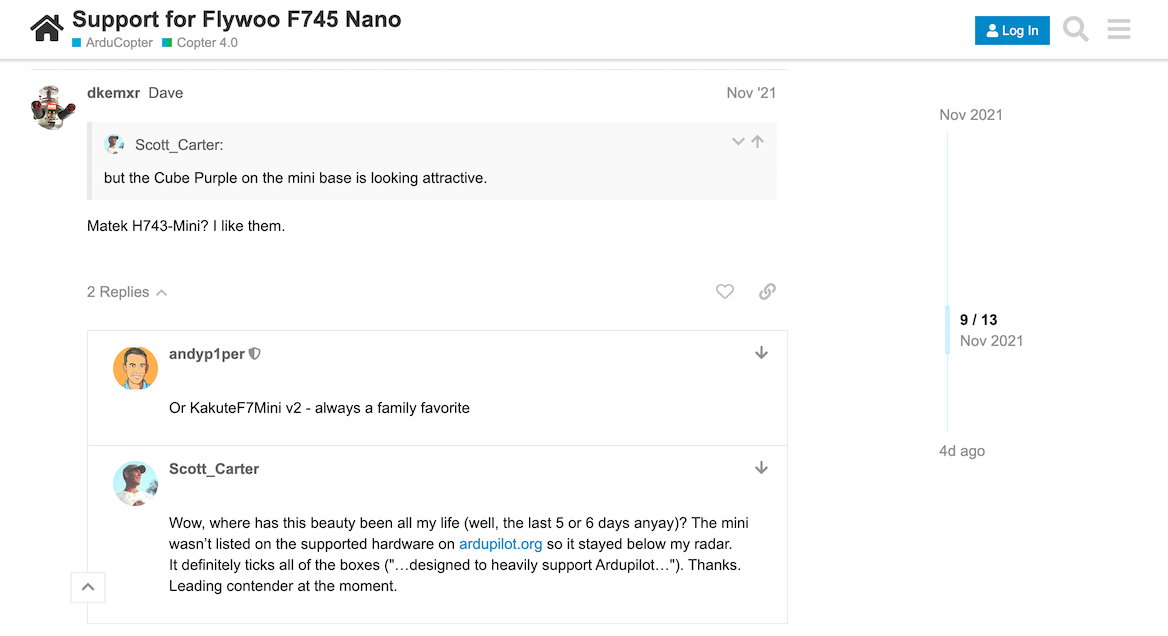
\includegraphics[width=\textwidth]{figures/data_collection/forum_topic_page}
        \caption{Topic Page}\label{fig:forum-topic-page}
    \end{center}
\end{figure}
The last layer consists of the topic page, the communication place between different users.
A user can create a new post or reply to an existing post.
For example, in \autoref{fig:forum-topic-page}, we can see the topic page for \qq{Support for Flywoo F745 Nano}.
Like the category page, it loads the posts dynamically when the user scrolls to the bottom.
However, the page only stores 25 posts per time in the \ac{HTML}.
Thus, if the user scrolls and loads new posts, previous loaded posts will unload.
Furthermore, the replies on the posts are only accessible by clicking on a \qq{Replies} button.
The knowledge contains in these communications.
Thus, we want to gather the textual context for all posts and their replies.
Having a direct way to access a specific post without dealing with the topic page's dynamic load and unload behavior would benefit an efficient web scraping solution.
Fortunately, there is a unique \ac{URL} representation for each post.
For example, \url{https://discuss.arupilot.org/t/support-foru-flywoo-f745-nano/77952/3} is the \ac{URL} for the third post for the topic \qq{Support for Flywoo F745 Nano}.
We can build such a \ac{URL} by knowing the position of the post on the topic page and the \ac{URL} of the topic page by ourselves.
We receive the topic page \ac{URL} from the category page and the category page \ac{URL} from the root page.
Thus, to build the \ac{URL} for a specific post, we have to go through all layers on the forum.

\subsection{Web Scraper System Overview}\label{subsec:building-the-web-scraper}
\begin{figure}
    \begin{center}
        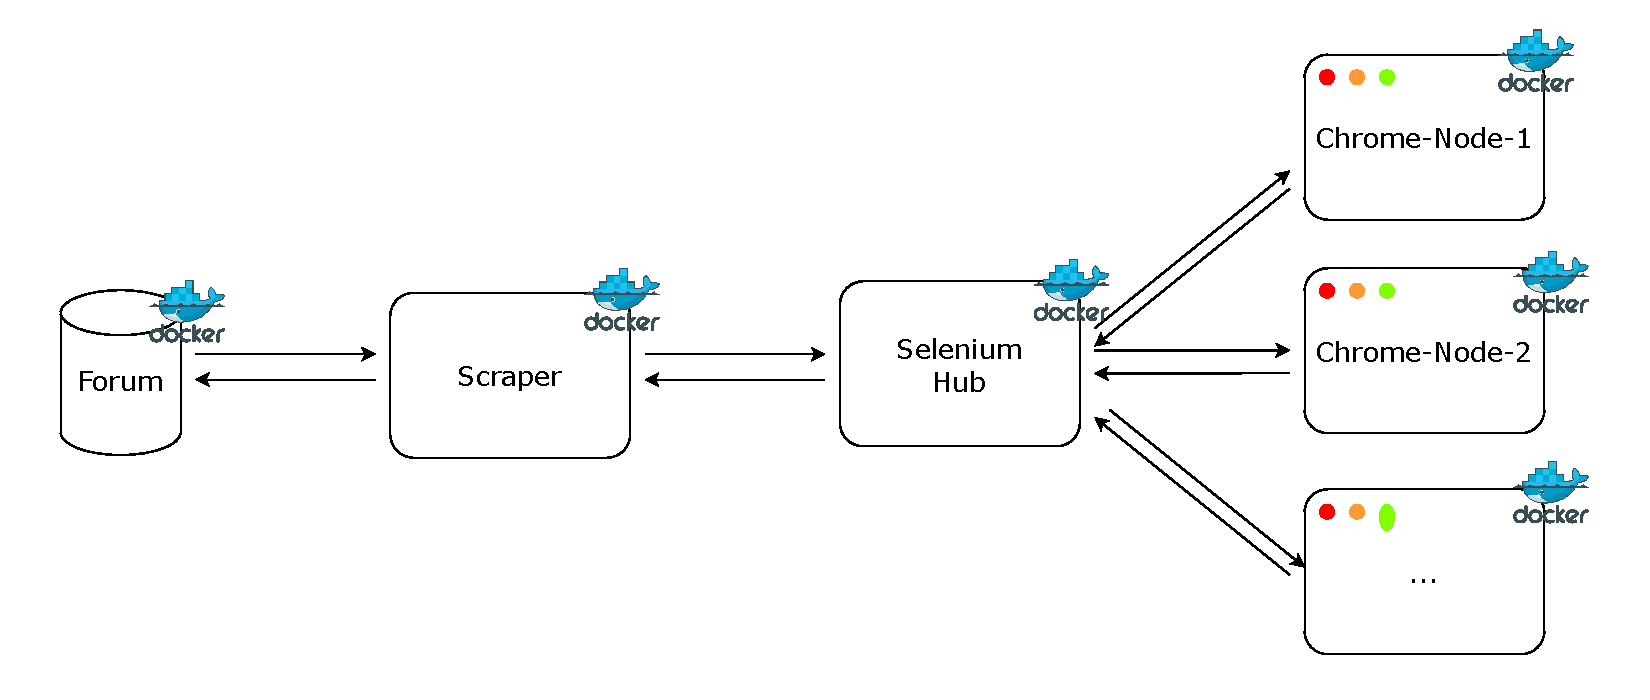
\includegraphics[width=\textwidth]{figures/data_collection/forum_scraper_architecture}
        \caption{Forum Web Scraper Architecture}\label{fig:forum-scraper-architecture}
        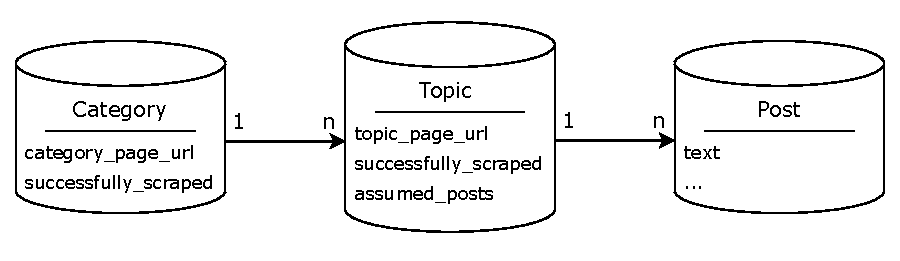
\includegraphics[scale=0.7]{figures/data_collection/forum_data_architecture}
        \caption{Forum Database Tables}\label{fig:forum-data-architecture}
    \end{center}
\end{figure}

This section provides an efficient, scalable, and robust way to access all posts and replies for these high dynamic webpages.
In \autoref{fig:forum-scraper-architecture} we can see the architecture of such a web scraper, consisting of at least four isolated docker\footnote{\url{https://www.docker.com/}} containers: a database, a web scraper, a hub, and multiple nodes, where the last two containers build a Selenium Grid\footnote{\url{https://github.com/SeleniumHQ/docker-selenium}}.
The first container hosts a PostgreSQL\footnote{\url{https://www.postgresql.org/}} database.
In \autoref{fig:forum-data-architecture} we can see the tables of the database, which are closely related to the page structure.
In the database, we store the scraped post contents and the \ac{URL}s for the different pages, information about the scraping status, and meta-information about the pages.
We use SQLAlchemy\footnote{\url{https://www.sqlalchemy.org/}}  to define our table schema and communicate with the PostgreSQL database.
The second container runs the web scraper.
The core of the scraper is the Selenium library which defines the logic for scraping new URLs or gathering content based on manually defined XPaths and CSS selectors.
We choose Selenium because it automates web browser interaction by communicating to the Selenium Grid.
We chose a Selenium Grid setup over a single web driver setup because it allows us to handle multiple web drivers parallel.
Furthermore, in combination with the Selenium Grid, Selenium allows us efficiently scroll down a page or click on a button, which is needed to access all topics on the category page or click on the \qq{Replies} button.

\subsection{Web Scraping Routine}\label{subsec:web-scraping-routine}
A docker-compose command triggers our web scraping routine after the Selenium Grid, and the database container is started.
We follow the layout structure of the discussion forum to gather all post \ac{URL}s.
First, we scrape the category page \ac{URL}s from the main page, which can be done by following the XPath to the corresponding \ac{HTML} elements.
Then we scrape for each category page all topic page URLs. Next, we use Selenium and the interaction with the web browser to scroll to the bottom of the category page to load all topics.
We store the topic page \ac{URL}s and the number of replies in the database.
The last step is to scrape all the posts by building unique post \ac{URL}s from the topic page \ac{URL} and the rank of the post on the page.
Using the number of replies, we know the upper bound of the possible ranks of the posts on a page.
Therefore, we can build all unique post \ac{URL}s by a simple loop over the number of replies, where the loop index is similar to the rank.
There is one significant speed improvement by using the dynamic behavior of the topic page, where 25 posts are loaded per request.
Thus, we can significantly speed up the scraping by generating each twenty-fifth \ac{URL} and scraping the content for the other posts at once.
Unfortunately, Selenium Grid can have a timeout exception after several hours of scraping, triggering a WebDriverException in Selenium.
To handle these errors, we wrap the previous scraping routine in a try-catch block which triggers a docker-compose restart when an exception occurs.
Thus, the scraping script will start from the beginning.
To continue the old progress, we store an additional attribute $scraped\_successfully$ to the category and topic table, which allows us to skip the pages marked as $scraped\_successfully$.
The previous steps allow us to scrape the dynamic discussion forum efficiently and robustly.


\section{Documentation}\label{sec:documentation}

\subsection{Structure Of The Documentation}\label{subsec:structure-of-the-documentation}
\begin{figure}
    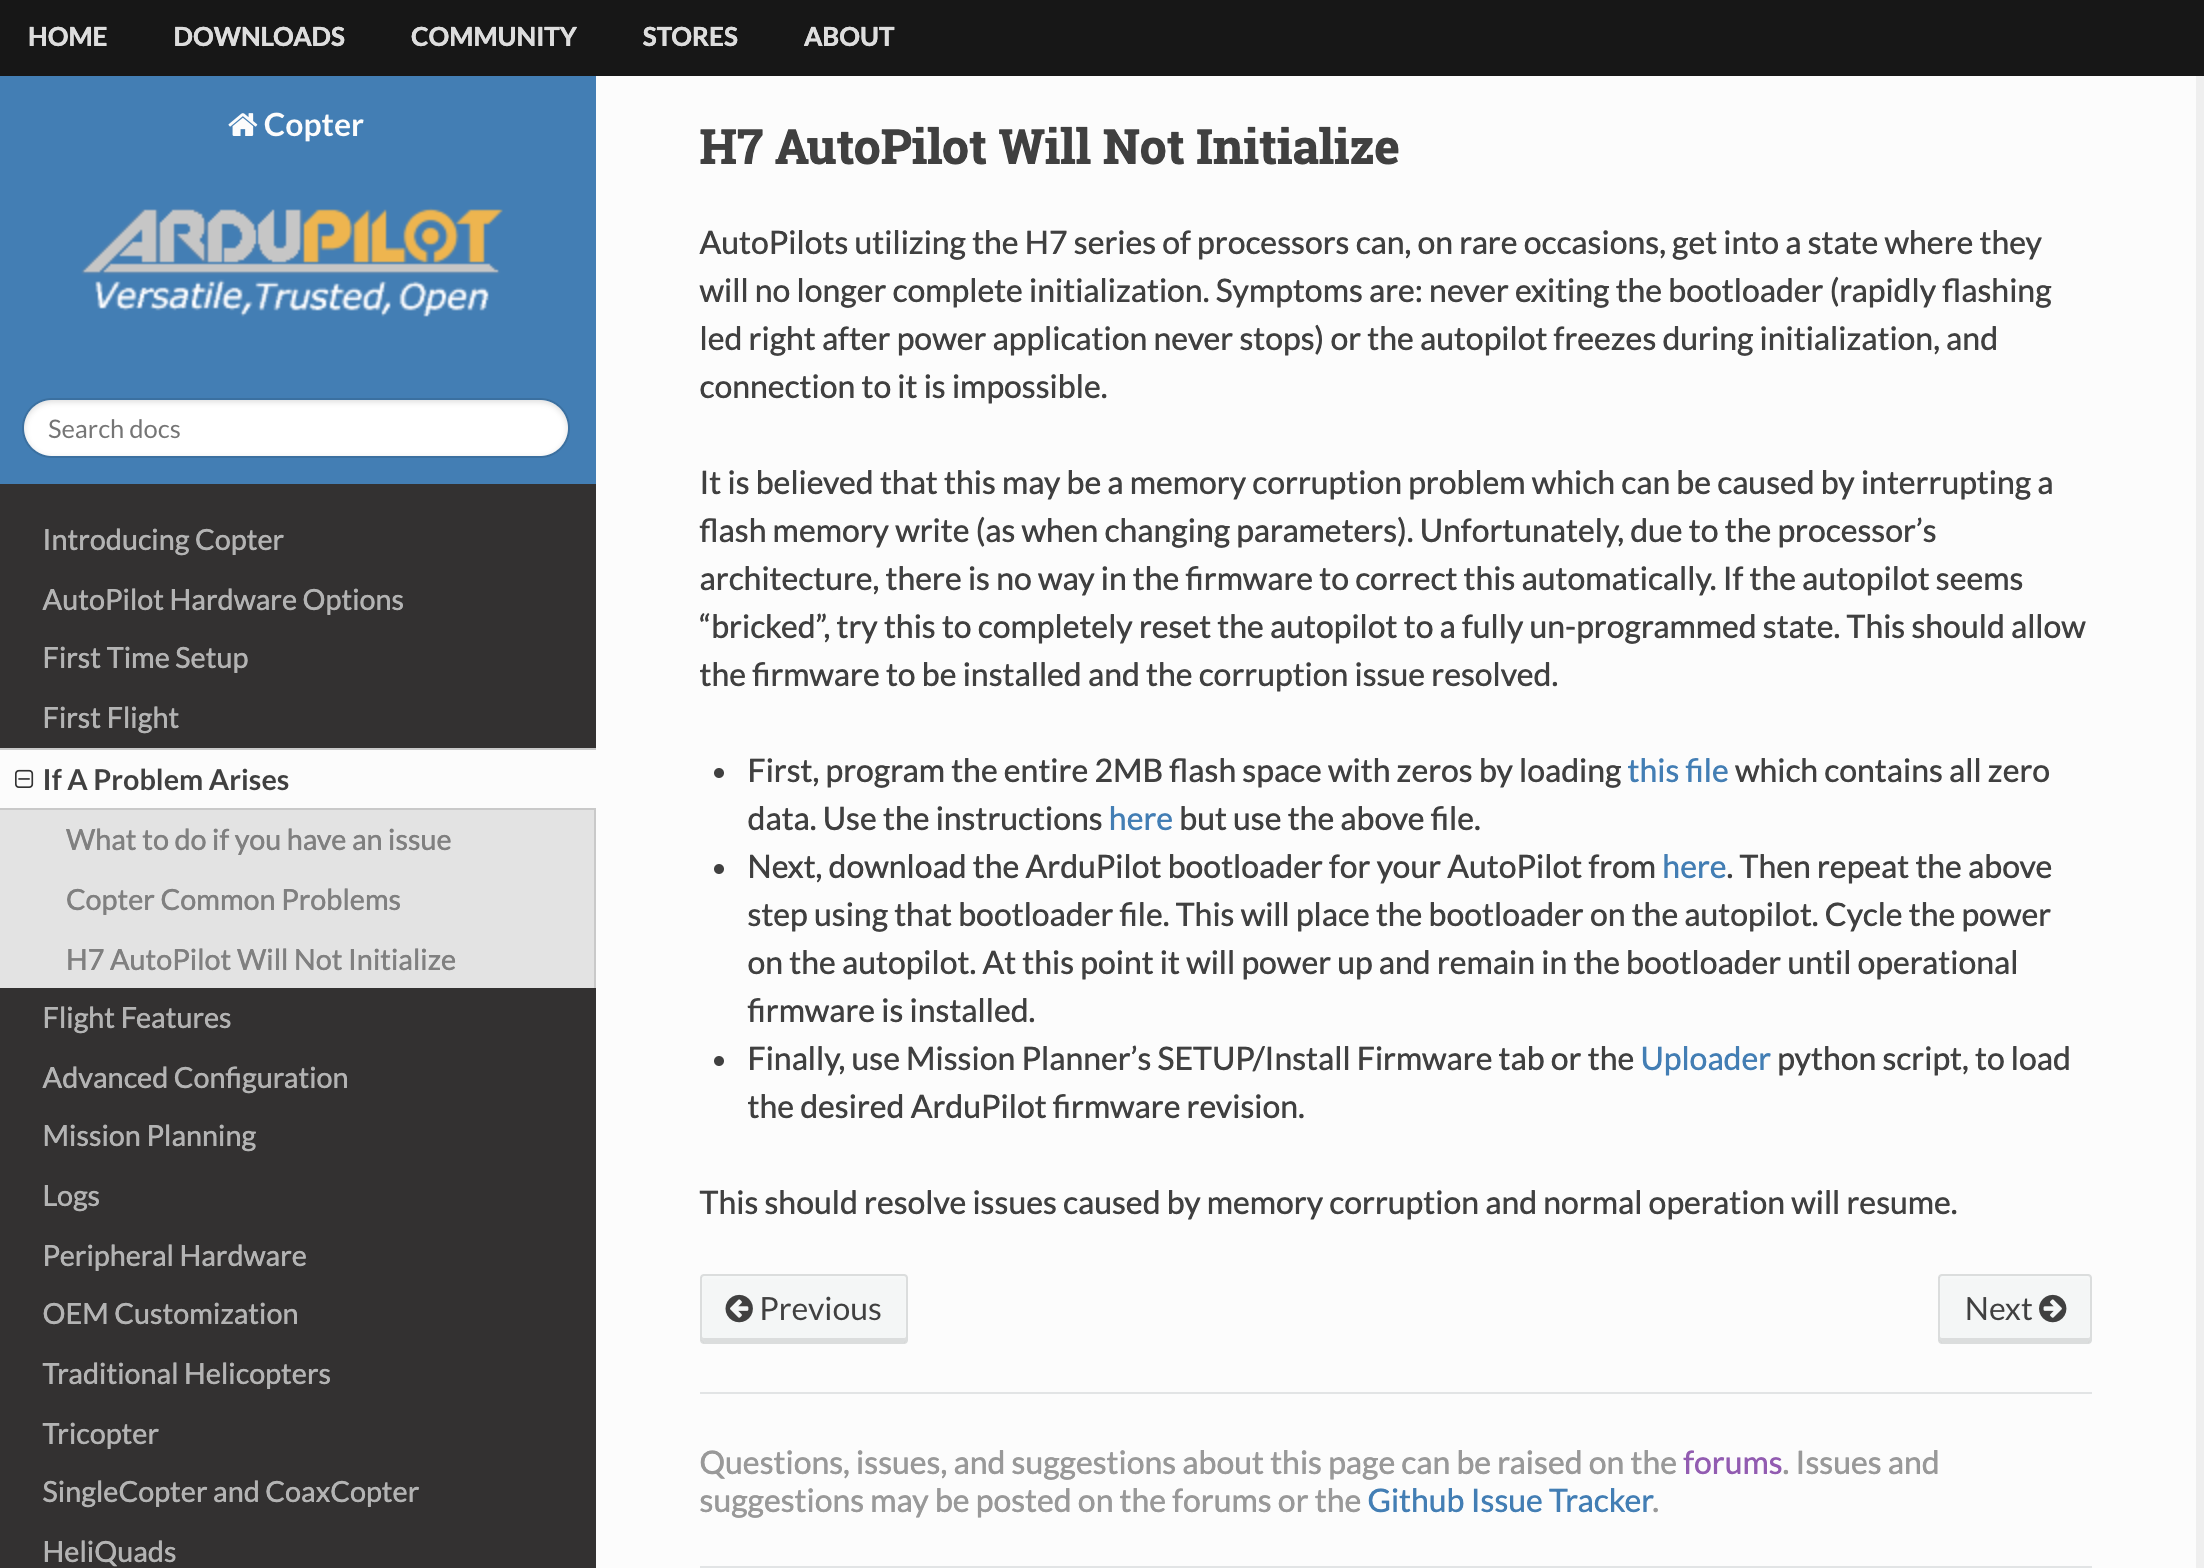
\includegraphics[width=\textwidth]{figures/data_collection/documentation_full_page}
    \caption{Documentation Page}\label{fig:documentation-full-page}
\end{figure}

Ardupilot provides online documentation about their software, which their developers maintain.
We also want to use this source because it is high quality and covers the ArduPilot system.
It also differs from the discussion forum and the discord chat in that the content is more structured with less noise which can be seen in \autoref{fig:documentation-full-page}.
The documentation consists of three main sections.
The first section is the navigation sidebar on the left, which gives an overview of all documentation topics.
The second section provides the content of a specific documentation page, which is loaded statically and therefore accessible without interacting with the page.
The last part consists of two buttons, \qq{Next} and \qq{Previous}, which allow navigating between the pages.
The documentation pages are fully connected, allowing it to access all documentation pages by only clicking on the \qq{Next} button when starting at the beginning.

\subsection{Scraping Strategy With Scrapy}\label{subsec:scrapy}
We decided to use Scrapy, a web crawling and scraping framework, to gather the structured data from the documentation page.
Scrapy uses spiders, which define how a specific site will be scraped, including how to perform the crawl and how to extract the data.
The spider acts in a cycle with the following steps:
\begin{enumerate}
    \item Start the scraping with an initial request to crawl the first \ac{URL} and define a callback function that handles the response.
    \item The callback function parses the page content using Selectors like XPath and combines the information into Scrapy items.
    We can also define a new request at the end of the callback function to build that cycle and repeat at 1).
    \item The items returned from the spider will be persisted in a database.
\end{enumerate}
We build a spider that starts at the root page of the documentation.
Next, we create a callback function that extracts the documentation page's textual content, which extracts the \ac{URL} from the \qq{Next} button.
Finally, we build the cycle by sending a new request with that \ac{URL} until we are at the end of the documentation.
Thus, we built a simple yet efficient and easily maintainable web scraper for online documentation.


\section{Discord}\label{sec:discord-webscraping}
The Discord platform is the main communication platform for the developers of the ArduPilot system.
There, the developers chat in different channels mainly about technical details and problems with the software.
Fortunate Discord provides a developer API\footnote{\url{https://discord.com/developers/docs/reference}} to scrape chat messages from channels directly.
We need to provide an authentication token in the request header to access the \ac{API}.
A simple GET request uses \url{https://discord.com/api/v9/channels/[channel_id]} as a \ac{URL} to access messages for a specific channel.
However, the Discord \ac{API} limits the number of response messages and returns only the latest messages.
Fortunate, we can specify path parameters to the GET request which looks like \url{https://discord.com/api/v9/channels/[channel_id]/messages?limit=[limit]&before=[before_id]}.
For the scope of our \ac{API} scraper, we only need to consider the $limit$ and the $before$ path parameter.
The $limit$ path parameter specifies the number of messages returned on a single request.
The default is 50, but it can be extended to 100 at most.
Furthermore, we can get older messages by setting the $before$ path parameter to some $messages\_id$.
Thus, we can build an efficient \ac{API} scraper that scrapes the messages from the channel, which consists of three parts:
\begin{enumerate}
    \item Send the initial request and specify the $channel\_id$ and the $limit$ path set to max.
    \item Extract the content of the message from the response and store the result in a database.
    \item If the response size is the same as the specified limit size, there are more messages in the chat.
    Thus, we extract the $message\_id$ from the last response item
    Finally, we send another request which specifies the $before$ parameter with the $message\_id$.
    We then continue at 2).
\end{enumerate}


\section{Merging And Cleaning}\label{sec:merging-and-cleaning}
The previous subsection described the different web scarping strategies for the ArduPilot channels.
Each of these scrapers produced a dataset containing raw textual information.
Unfortunately, the characteristics of the sources lead to a \qq{dirty} data source.
There are several reasons for the poor data quality in chat-based environments, which are closely connected to the user's behavior in online communication''
\begin{itemize}
    \item One logical sentence could be split into different paragraphs, which happens when a user places images inside a sentence or starts a new line accidentally.
    \item Extensive usage of a short text that includes no information like \qq{Hi}, \qq{no} or \qq{that's true}.
    \item The text contains special characters, e.g., smileys or links to other chat messages, users, or channels represented with their ids like \qq{@483512342}.
\end{itemize}

\subsection{Cleaning And Extracting Sentences}\label{subsec:cleaning-and-extracting-sentences}
We provide a pipeline that extracts correct, formatted, and cleaned sentences from raw textual data, implementing four steps:
\begin{enumerate}
    \item Preprocessing with regular expression: In the first step, we convert the raw text into an ASCII representation of the text and substitute the whitespace characters like $\setminus n$, $\setminus t$ or a sequence of whitespaces with a simple whitespace character.
    Additionally, the domain requires specific regular expression substitutions to handle $user\_id$s or links to other \ac{URL}s, which do not provide information.
    We could either drop such an occurrence or replace it with something meaningful.
    We decided to replace it with a generic representation like \qq{User} or \qq{URL} to maintain the structure of the sentence.
    \item Sentence segmentation: The following step was to extract the sentences from the pre-processed text.
    We could create a bunch of regular expression rules to find the boundaries of a sentence.
    However, the sentences could be represented ambiguously, and the users could format or mark the start and end of a sentence that is not reflected in our patterns.
    Therefore, we decided to use the spaCy\footnote{\url{https://spacy.io/}} library to detect sentence boundaries based on a pre-trained \ac{NLP} model (see \autoref{ch:cause-effect-extraction}).
    These extracted sentences do not necessarily have to end with punctuation or start with an uppercase.
    Therefore, we substituted the first character with an uppercase and added punctuation.
    \item Grammar checker: The sentence segmentation also extracts short sentences without information such as \qq{Hi!} or \qq{That is true}.
    We do not want to include such sentences in the resulting dataset.
    Thus, we decided to drop sentences that do not meet the standards for a complete sentence, which means that we drop sentences without a verb, an object, or a subject.
    \item Remove duplicate mentions: It is common to reference other messages or posts in a chat-based environment.
    In \autoref{fig:forum-topic-page} we can see an example of such a reference.
    When a user references another post, the content of the reference will be injected into the user's post.
    Thus, we have duplicate sentences that are from the same source.
    Hence, we decided to drop such sentences.
\end{enumerate}

\subsection{Merging Into One Source}\label{subsec:merging-to-one-source}
The last step of the data collection pipeline is to combine the extracted sentences from the different sources into one source.
We decided to combine everything into a single CSV file because it makes it easier to explore the dataset and share it with other researchers.
The dataset consists of three columns:
\begin{itemize}
    \item id - integer: A unique identifier for a sentence which is especially useful when you want to backtrack the sentence at the different pipeline stages.
    \item sentence - string: A sentence that is mentioned by a domain expert from the Ardupilot community.
    \item source - string: A categorical variable that is either \qq{forum}, \qq{docs} or \qq{chat}, which indicates the source of the sentence.
\end{itemize}
This dataset represents the domain-expert knowledge about the users and developers of the Ardupilot system.
